\documentclass[english]{tktltiki}
\usepackage[pdftex]{graphicx}
\usepackage{subfigure}
\usepackage{enumerate}
\usepackage[table,xcdraw]{xcolor}
\begin{document}
\onehalfspacing

\title{Location Awareness - Week 6}
\author{P�ter Ivanics}
\date{\today}

\maketitle

\numberofpagesinformation{\numberofpages\ pages + \numberofappendixpages\ appendices}
\keywords{}

\mytableofcontents

\section{Course feedback}
	The topics and the objectives of the course are very interesting and highlight relevant problems of the present time. The topics are extensive, deep and the material provides good understanding on the covered topics. The lecturers did an extremely good job and invested a lot of time to prepare the material and design the contents of the course. 
	
	The objectives, tasks and required effort from the students' side were stated well in advance of the course. We were informed what is required from us and how the evaluation system will work. The lectures were well structured, however often times the topics were very deep and difficult to follow. I believe the lectures could be made a bit better by dedicating some time to introduce the basic concepts in more depth and maybe by involving the audience more. Some group exercises on the lectures could be useful. 
	
	The exercises were on a good level of difficulty most of the time. Personally found the Kalman filter (Week 4) and the Week 5 exercise set the most demanding. Despite the fact that the description of the exercises was understandable, I would suggest to add some hints or more explanations to these tasks at least. 
	
	In comparison to other courses, this one takes quite a lot of effort and I think it would worth 6 credit points even without the project work. I am not sure if it would be possible, but some students might appreciate to do the project "optionally" for 1-2 credits separately. 
	
	Finally, I would like to mention that the contents of this course is strongly correlated and very similar in some cases with the topics covered in the Introduction to Machine Learning course ongoing in the same semester. For me it was very good to take these courses at the same time, because I had the chance to practice more or less the same topics. Nevertheless, both courses build on strong mathematical and statistical basis in many cases, which I personally should improve - maybe this could be pointed out next time as others may face the same issue.

\section{Trajectory Similarity Measures}
	\begin{enumerate}[a)]
		\item Dynamic Time Warping (DTM) and Longest Common SubSequence (LCSS) are both similarity measures for trajectory of objects. They are both carried out as a dynamic programming algorithm in practice, but their approach to the similarity measure is fundamentally different. DTM measures the dissimilarity between objects (strings), while LCSS seeks similarities in the trajectories. On one hand, DTW takes time differences into consideration, while LCSS has the capability to completely remove patterns/outliers from the measurements. Neither of these two methods are metric, which is their common disadvantage. 
		\item To cluster movement trajectories of animals, I would use the LCSS technique. As we are interested in modeling the group of animals wandering together between locations, an algorithm that identifies the similarities in the trajectories and ignores outliers is needed. LCSS is an appropriate choice as it ignores non-matching parts and reduces the noise (in this case individual animals leaving the herd) from the data.
		\item In this case I would suggest to use DTW, because that would help to indicate the differences/dissimilarity of the measurements numerically. As the penalties are determined between the points as the (Eucledian) distance, it would serve as a good indication measuring the difference between trajectories. 
		\item Fre?chet distance is another measure which can estimate similarity of two curves or trajectories. This measure is also called a "dog leash" distance. This metaphor is explained by the fact that the Fre?chet distance is defined by the minimum distance (length of the dog leash) that is required to connect two discrete points of on the two curves (the dog and its owner). Some call this measure as coupling distance because it examines the coupling of discrete points. In the scope of this course and Location Awareness is technique interesting because it is another way to measure trajectory similarities. 
	\end{enumerate}

\section{Dynamic programming}
\begin{enumerate}[a)]
	\item The edit distance of the given strings is $3$. The edit matrix is displayed in Table \ref{editmatrix}.
	
	\begin{table}[]
\centering
\caption{The calculated distances for the given strings to determine the edit distance. The red numbers indicate the backtracking route.}
\label{editmatrix}
\begin{tabular}{llllllllll}
\hline
           &                          & \textbf{G}               & \textbf{A}               & \textbf{R}               & \textbf{G}               & \textbf{A}               & \textbf{M}               & \textbf{E}               & \textbf{L}               \\
           \hline
           & {\color[HTML]{FE0000} 0} & 1                        & 2                        & 3                        & 4                        & 5                        & 6                        & 7                        & 8                        \\
\textbf{C} & 1                        & {\color[HTML]{FE0000} 2} & 3                        & 4                        & 5                        & 6                        & 7                        & 8                        & 9                        \\
\textbf{A} & 2                        & 3                        & {\color[HTML]{FE0000} 2} & 3                        & 4                        & 5                        & 6                        & 8                        & 8                        \\
\textbf{R} & 3                        & 4                        & 3                        & {\color[HTML]{FE0000} 2} & {\color[HTML]{FE0000} 3} & 4                        & 5                        & 6                        & 7                        \\
\textbf{A} & 4                        & 5                        & 4                        & 3                        & 4                        & {\color[HTML]{FE0000} 3} & 4                        & 5                        & 6                        \\
\textbf{M} & 5                        & 6                        & 5                        & 4                        & 5                        & 4                        & {\color[HTML]{FE0000} 3} & 4                        & 5                        \\
\textbf{E} & 6                        & 7                        & 6                        & 5                        & 7                        & 5                        & 4                        & {\color[HTML]{FE0000} 3} & 4                        \\
\textbf{L} & 7                        & 8                        & 7                        & 6                        & 7                        & 6                        & 5                        & 4                        & {\color[HTML]{FE0000} 3} \\
\hline
\end{tabular}
\end{table}
	\item The Longest Common SubSequence of the strings CARAMEL and GARGAMEL are, as follows: 
		\begin{eqnarray*}
			LCSS("CARAMEL", "GARGAMEL") = "ARAMEL"
		\end{eqnarray*}
		
		The calculated matrix for and the backtracking is displayed in Table \ref{lcss}.
		
		\begin{table}[]
\centering
\caption{The calculated distances for the given strings to determine the Longest Common SubSequence. The red numbers indicate the backtracking route.}
\label{lcss}
\begin{tabular}{lllllllll}
\hline
           & \textbf{G}               & \textbf{A}               & \textbf{R}               & \textbf{G} & \textbf{A}               & \textbf{M}               & \textbf{E}               & \textbf{L}               \\
           \hline
\textbf{C} & {\color[HTML]{FE0000} 0} & 0                        & 0                        & 0          & 0                        & 0                        & 0                        & 0                        \\
\textbf{A} & 0                        & {\color[HTML]{FE0000} 1} & 1                        & 1          & 1                        & 1                        & 1                        & 1                        \\
\textbf{R} & 0                        & 1                        & {\color[HTML]{FE0000} 2} & 2          & 2                        & 2                        & 2                        & 2                        \\
\textbf{A} & 0                        & 1                        & 2                        & 2          & {\color[HTML]{FE0000} 3} & 3                        & 3                        & 3                        \\
\textbf{M} & 0                        & 1                        & 2                        & 2          & 3                        & {\color[HTML]{FE0000} 4} & 4                        & 4                        \\
\textbf{E} & 0                        & 1                        & 2                        & 2          & 3                        & 4                        & {\color[HTML]{FE0000} 5} & 5                        \\
\textbf{L} & 0                        & 1                        & 2                        & 2          & 3                        & 4                        & 5                        & {\color[HTML]{FE0000} 6} \\
\hline
\end{tabular}
\end{table}
	\item The Eucledian distances between the points are displayed in Table \ref{distances}. The DTW value respectively is the value 
	
	\begin{equation}
		dist(C, G) + dist(C, G) + dist(R, G) = 0.41 + 0.41 + 0.72 = 1.54
	\end{equation}
	
	\begin{table}[ht]
\centering
\caption{The Eucledian distances between the given points.}
\label{distances}
\begin{tabular}{rrrrrrrr}
  \hline
 & C & A & R & M & E & L & G \\ 
  \hline
  C & 0.00 & 0.58 & 0.76 & 0.74 & 0.55 & 0.23 & 0.41 \\ 
  A & & 0.00 & 0.92 & 0.16 & 0.09 & 0.39 & 0.22 \\ 
  R &  & & 0.00 & 0.99 & 0.83 & 0.86 & 0.72 \\ 
  M & & & & 0.00 & 0.20 & 0.54 & 0.36 \\ 
  E & & & &  & 0.00 & 0.38 & 0.15 \\ 
  L & &  & & & & 0.00 & 0.28 \\ 
  G & & & & & & & 0.00 \\ 
   \hline
\end{tabular}
\end{table}
\end{enumerate}

\section{Trajectory Clustering}
	\begin{enumerate}[a)]
		\item The $loadPrunedMeasurements()$ function in the attached $trajectory\_clustering.R$ script performs the pruning of the points. The pruned points (6806) in total are visualized Figure \ref{coordinates}.

		\begin{figure}[h] 
		\begin{center}
			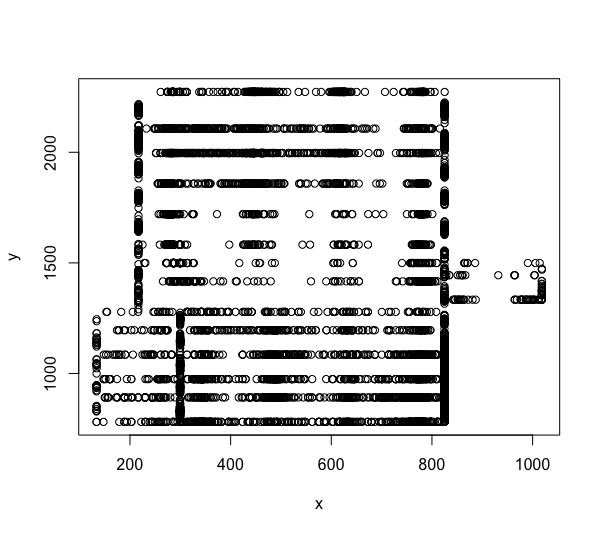
\includegraphics[width=0.8\textwidth]{images/coordinates.png}
			\caption{The scatter plot of the coordinates for Task 4.}
			\label{coordinates}
		\end{center}
	\end{figure}			
		
		\item 
	\end{enumerate}
\nocite{*}
\bibliographystyle{tktl}
\bibliography{lahteet}

\lastpage

\pagestyle{empty}

\end{document}